\documentclass[dvipdfmx,uplatex]{jsarticle}
\usepackage{amsmath,amssymb,amsfonts}
\usepackage{setspace}
\usepackage{empheq}
\usepackage{tikz}
\usepackage{here}
\usepackage{listings, jlisting}
\lstset{
  language=html,
  basicstyle=\ttfamily\scriptsize,
  commentstyle=\textit,
  classoffset=1,
  keywordstyle=\bfseries,
  frame=tRBl,
  framesep=5pt,
  showstringspaces=false,
  numbers=left,
  stepnumber=0,
  numberstyle=\tiny,
  tabsize=2,
  breaklines = true,
}

\title{確率論第1回演習課題}
\author{長田悠生}
\date{2023/4/22}


\begin{document}
  \begin{titlepage}
    \maketitle
    \begin{center}
      \textmc{\HUGE \LaTeX}
    \end{center}
    \thispagestyle{empty}
  \end{titlepage}

  \centerline{\huge 演習課題1A}
  \vspace{10mm}
  \textmc{まずは、問題文の理解のためにHTML・CSS風に構造化してみる。\\}
  \textmc{\large HTML}
  \begin{lstlisting}
<全体の問題文 class="全体の問題文">
  <(a) class="全体の問題文">
    この国の王位継承は女性が優先される場合に,きょうだいが男性である確率を求めよ.
  </(a)>
  <(b) class="全体の問題文">
    この国では年長者が王位を継承する場合に,きょうだいが男性である確率を求めよ.
  </(b)>
</全体の問題文>
  \end{lstlisting}

  \textmc{\large CSS}
  \begin{lstlisting}
.全体の問題文 {
  ある国の女王には,きょうだいが一人いる;
  なお(a), (b)において,この国では男女の生まれる確率は等しいとする;
}
  \end{lstlisting}
  \textmc{問題文についての理解を深めたところで、問題を解いていく。\\}
  \begin{spacing}{1.3}
    \textmc{\large (a)\\}
  \end{spacing}
  \textmc{ある国にいる二人の人(問題文での女王とその兄弟一人)について、男・女の観点における全パターンを標本空間として問題を解く。\\}
  \begin{equation}
    \Omega = \{女女、男女、女男、男男\}
  \end{equation}
  \textmc{二人のうち少なくともどちらか一方が女である場合を、事象Aとする。また、きょうだいが男である場合を、事象Bとする。\\}
  \begin{spacing}{1.3}
    \textmc{条件付き確率の定義 \\}
  \end{spacing}
  \begin{equation}
    P(B|A)=\frac{P(A \cap B)}{P(A)}
  \end{equation}
  \textmc{に従い計算を行う。\\}
  \textmc{標本空間において、事象Aが発生する確率は、\\}
  \begin{equation}
    事象Aの確率=\frac{3}{4}
  \end{equation}
  \textmc{$A \cap B$の事象は女男か男女になる確率だから、 \\}
  \begin{equation}
    事象A \cap Bの確率=\frac{1}{2}
  \end{equation}
  \textmc{よって、 \\}
  \begin{equation}
    P(B|A)=\cfrac{\;\cfrac{1}{2}\;\;}{\;\cfrac{3}{4}\;\;}=\frac{2}{3}
  \end{equation}

  \begin{spacing}{1.3}
    \textmc{\large (b)\\}
  \end{spacing}
  \textmc{ある国にいる二人の人(問題文での女王とその兄弟一人)をそれぞれA, Bとする。このとき、A, Bについて性別・年上・年下の観点における全パターンを標本空間として問題を解く。\\}

  \begin{empheq}[left={\Omega=\empheqlbrace},right={\empheqrbrace}]{alignat=4}
    A(年上・男) B(年下・女)、A(年下・男) B(年上・女) \\
    A(年上・男) B(年下・男)、A(年下・男) B(年上・男) \\
    A(年上・女) B(年下・女)、A(年下・女) B(年上・女) \\
    A(年上・女) B(年下・男)、A(年下・女) B(年上・男)
  \end{empheq}
  \textmc{Aが王位を継承する場合を、事象$\alpha$とする。また、Bが男である場合を、事象$\beta$とする。\\}
  \begin{spacing}{1.3}
    \textmc{条件付き確率の定義 \\}
  \end{spacing}
  \begin{equation}
    P(\beta|\alpha)=\frac{P(\alpha \cap \beta)}{P(\alpha)}
  \end{equation}
  \textmc{に従い計算を行う。\\}
  \textmc{標本空間において、事象$\alpha$が発生する確率は、\\}
  \begin{equation}
    事象 \alpha の確率=\frac{1}{2}
  \end{equation}
  \textmc{$\alpha \cap \beta$の確率は、 \\}
  \begin{equation}
    事象 \alpha \cap \beta の確率=\frac{1}{2} \times \frac{1}{2} = \frac{1}{4}
  \end{equation}
  \textmc{よって、 \\}
  \begin{equation}
    P(\beta|\alpha)=\cfrac{\;\cfrac{1}{4}\;\;}{\;\cfrac{1}{2}\;\;}=\frac{1}{2}
  \end{equation}
  \textmc{Aが王位を継承する場合もBが王位を継承する場合も同様の確率になる。\\}
  \textmc{この問題において、A・Bの区別を対象の二人につけていないので、この問題の答えは$\frac{1}{2}$となる。\\}

  
  \centerline{\huge 演習課題1B}
  \vspace{10mm}
  \begin{center}
    \textmc{$P(A \cap B|C)$をベン図で表現すると以下のようになる。\\}
    \textmc{注) 以下の図は、簡略化の為にCを消している。\\}
  \end{center}
  \begin{figure}[H]
    \centering
    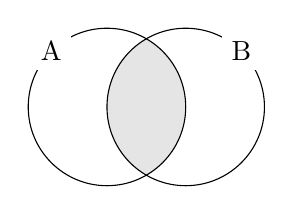
\begin{tikzpicture}
      \begin{scope} \clip (1,0) circle [radius=1];
        \fill[black!10!] (0,0) circle [radius=1];
      \end{scope}
      \draw (0,0) circle [radius=1];
      \draw (1,0) circle [radius=1];
      \draw ({cos(pi*3/4 r)},{sin(pi*3/4 r)}) node[fill=white]{A};
      \draw ({1+cos(pi/4 r)},{sin(pi/4 r)}) node[fill=white]{B};
    \end{tikzpicture}
  \end{figure}

  \begin{center}
    \textmc{$P(A \cap B^c|C)$をベン図で表現すると以下のようになる。\\}
    \textmc{注) 以下の図は、簡略化の為にCを消している。\\}
  \end{center}
  \begin{figure}[H]
    \centering
    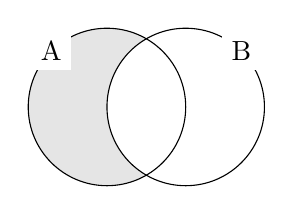
\begin{tikzpicture}
      \begin{scope} \clip (0,0) circle [radius=1];
        \fill[black!10!] (0,0) circle [radius=1];
        \fill[white!] (1,0) circle [radius=1];
      \end{scope}
      \draw (0,0) circle [radius=1];
      \draw (1,0) circle [radius=1];
      \draw ({cos(pi*3/4 r)},{sin(pi*3/4 r)}) node[fill=white]{A};
      \draw ({1+cos(pi/4 r)},{sin(pi/4 r)}) node[fill=white]{B};
    \end{tikzpicture}
  \end{figure}

  \begin{center}
    \textmc{以上より、$P(A \cap B|C) + P(A \cap B^c|C)$をベン図で表現すると以下のようになる。\\}
    \textmc{注) 以下の図は、簡略化の為にCを消している。\\}
  \end{center}
  \begin{figure}[H]
    \centering
    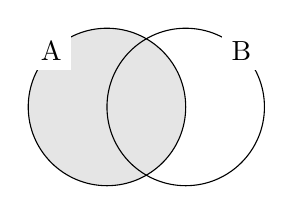
\begin{tikzpicture}
      \begin{scope} \clip (0,0) circle [radius=1];
        \fill[black!10!] (0,0) circle [radius=1];
      \end{scope}
      \draw (0,0) circle [radius=1];
      \draw (1,0) circle [radius=1];
      \draw ({cos(pi*3/4 r)},{sin(pi*3/4 r)}) node[fill=white]{A};
      \draw ({1+cos(pi/4 r)},{sin(pi/4 r)}) node[fill=white]{B};
    \end{tikzpicture}
  \end{figure}

  \textmc{よって、$P(A \cap B|C) + P(A \cap B^c|C) = P(A|C)$}

\end{document}